% Klassifiziert den Dokumenten-Typ
% Doku: http://exp1.fkp.physik.tu-darmstadt.de/tuddesign/
% Farben: http://www.tu-darmstadt.de/media/medien_stabsstelle_km/services/medien_cd/das_bild_der_tu_darmstadt.pdf
%  bigchapter: Chapter haben doppelte Schriftgröße
%  linedtoc: Linien im Inhaltsverzeichnis wie bei Überschriften
%  colorbacktitle: Der Dokumenten-Titel wird mir der Accentfarbe hinterlegt
\documentclass[bigchapter,colorback,accentcolor=tud4b,linedtoc,11pt]{tudreport}

% Input Dokument hat das Encoding UTF-8
\usepackage[utf8]{inputenc}
% Wichtiges Paket für Links und verlinktes Inhaltsverzeichnis
\usepackage[ngerman]{hyperref}
% Paket für Fußnoten
\usepackage[stable]{footmisc}
% Paket für Bibliotheks-Verzeichnis, square: Verwende eckige statt runde klammern
% \usepackage[square]{natbib}
% Paket zum Plotten von Datensätzen
\usepackage{pgfplots}
\usepackage{textcomp}
% Verwende deutsche Bezeichner für Inhaltsverzeichnis, ... (ngerman = New German: neue Rechtschreibung)
\usepackage{ngerman}
% Modul für chemische Formeln
%\usepackage{chemformula}
% Deutsche Zahlen (entfernt z.B. das Leerzeichen nach einem Dezimal-Komma)
\usepackage{ziffer} 
%wegen Grafikverschiebung hinzugefügt
\usepackage{float}

\usepackage[verbose]{placeins}

%\usepackage{graphicx}
%\usepackage{caption}
\usepackage{subcaption} %Für subfigures

% Anhänge für Original-Messdaten
\usepackage{fancyvrb}

% redefine \VerbatimInput
\RecustomVerbatimCommand{\VerbatimInput}{VerbatimInput}%
{fontsize=\footnotesize,
 %
 frame=lines,  % top and bottom rule only
 framesep=2em, % separation between frame and text
 fontsize=\scriptsize,
 %
 labelposition=topline,
 %
 commandchars=\|\(\), % escape character and argument delimiters for
                      % commands within the verbatim
 commentchar=*        % comment character
}

\pgfkeys{%
  /pgfplots/epsilonforuf/.style={%
    legend pos=north west,
    xlabel=$U_m$  in  $V$,
    x tick label style={/pgf/number format/.cd,%
      set thousands separator={},
      set decimal separator={,}
    },%
    ylabel=Beugungseffizienz $\varepsilon$,
    y tick label style={/pgf/number format/.cd,%
      set thousands separator={},
      set decimal separator={,}
    },%
    width=0.38\linewidth,
    height=0.22\linewidth,
    scale only axis,
    xmin=0,
    xmax=5,
    grid=both,
    ymin=0,
    ymax=0.82,
    tick align=outside,
    tickpos=left,
    minor x tick num=3,
    minor y tick num=4,
    minor grid style={dotted,thin},
  }
}

\pgfkeys{%
  /pgfplots/epsilonfortheta/.style={%
    legend pos=north east,
    xlabel=$\theta$  in  Grad,
    x tick label style={/pgf/number format/.cd,%
      set thousands separator={},
      set decimal separator={,}
    },%
    ylabel=Beugungseffizienz $\varepsilon$,
    y tick label style={/pgf/number format/.cd,%
      set thousands separator={},
      set decimal separator={,}
    },%
    width=0.38\linewidth,
    height=0.22\linewidth,
    scale only axis,
    xmin=0,
    xmax=0.9,
    grid=both,
    ymin=0,
    ymax=0.92,
    tick align=outside,
    tickpos=left,
    minor x tick num=3,
    minor y tick num=4,
    minor grid style={dotted,thin},
  }
}

% PDF-Optionen
\hypersetup{%
  pdftitle={TU Darmstadt \- Physikalisches Praktikum für Fortgeschrittene},
  pdfauthor={Esra Bauer und Sören Link},
  pdfsubject={Versuch 4.10},
  pdfview=FitH,
}

% Kleines makro zur assymetrischen Fehlerangabe
\def\tol#1#2#3{\hbox{\rule{0pt}{15pt}${#1}^{+{#2}}_{-{#3}}$}}% 

% Entspricht-Zeichen
\usepackage{scalerel}

\newcommand\equalhat{%
\let\savearraystretch\arraystretch
\renewcommand\arraystretch{0.3}
\begin{array}{c}
\stretchto{
    \scalerel*[\widthof{=}]{\wedge}
    {\rule{1ex}{3ex}}%
}{0.5ex}\\ 
=%
\end{array}
\let\arraystretch\savearraystretch
}
%BEGINN TITELSEITE

\title{Akusto-optischer Modulator}

\subtitle{Esra Bauer  \\Sören Link}

\subsubtitle{Betreuer: Daniel Schraft \hfill Versuchsdatum: 8. Dezember 2014}

\author{Esra Bauer, Sören Link}

%\settitlepicture{img/title.jpg}

\institution{Physikalisches Praktikum \\für Fortgeschrittene \\ Versuch 4.10}

\date{\today}


%ENDE TITELSEITE

\begin{document}
%ANFANG DOKUMENT

%Titelseite einfügen
\maketitle

%Inhaltsverzeichnis einfügen
\tableofcontents

%ANFANG INHALT

\chapter{Einleitung}

In diesem Versuch soll der akusto-optische Effekt untersucht werden und durch die Inbetriebnahme eines akusto-optischen Modulators auf verschiedene Arten angewendet werden. Entscheidend ist dabei die Wechselwirkung von Licht- und Schallwellen (im Versuch werden Ultraschallwellen eingesetzt), die es ermöglicht, dass Licht an Schallwellen wie an einem Kristall gebeugt wird. Akusto-optische Modulatoren sind heute u.a.\ wichtige Elemente der Forschung (z.b. Spektroskopie, Bose-Einstein-Kondensation) und der Telekommunikation sowie der Quantenoptik, um nur einige Einsatzgebiete zu nennen. Es können auch Laserpulse erzeugt werden und vieles mehr, was teilweise im Versuch umgesetzt bzw.\ aufgezeigt wird.

\chapter{Grundlagen}
\section{Akusto-optischer Effekt}

Der akusto-optische Modulator (AOM) nutzt die Tatsache, dass Schallwellen in einem Medium ein optisches Gitter erzeugen. Sie bewirken eine periodische Dichte- und somit Brechnungsindexmodulation, d.h.\ es entsteht ganz analog zur Bragg-Reflexion ein Gitter mit der ``Gitterkonstanten'' $\lambda_S$, der Schallwellenlänge. Es gilt folglich für konstruktive Interferenz: 
$$2~sin(\theta) = \frac{\lambda}{\lambda_S}$$ 
Zur technischen Umsetzung dient ein an einen Tellurdioxid-Kristall montierter Piezo-Aktor, welcher beim Anlegen einer geeigneten Hochfrequenzspannung entsprechende mechanische Schwingungen ausführt. Auf der gegenüberliegenden Seite ist ein Absorber zur Verhinderung stehender Wellen angebracht.

\section{Betriebsregime eines AOMs}

Die Bragg-Bedingung setzt bei genauer Betrachtung eine hinreichende Länge des Mediums voraus, durch welches die Schallwelle propagiert und eine Brechungsindexmodulation bewirkt. Es tritt dann nur die erste Beugungsordnung auf und man spricht vom Bragg-Regime. Dies liegt auch unserer Betrachtung zugrunde, man muss aber beachten, dass auch das sog. Raman-Nath (häufig auch: Debye-Sears-Regime) vorliegen kann, vor allem wenn die Länge des Mediums kurz im Vergleich zur Schallwellenlänge ist. Die Bragg-Bedingung gilt dann nicht mehr, d.h.\ es tritt keine klassische Beugung am Gitter auf, sondern lediglich eine periodische Veränderung der Phase des Lichts. Es sind dann auch höhere Beugungsordnungen zu beobachten. Zur Unterscheidung kann ein Parameter $\rho$ wie folgt definiert werden: 
$$\rho = \frac{\lambda_0^2}{\lambda_S~\bar{n}~n_1}$$
$\lambda_0$ ist dabei die Lichtwellenlänge im Vakuum, $\bar{n}$ der mittlere Brechnungsindex und $n_1$ die Modulation des Brechnungsindex. Gilt $\rho \gg 1$ (etwa ab 10), kann man vom Bragg-Regime ausgehen, für $\rho \leq 1$ vom Raman-Nath-Regime.

\section{Doppelpasskonfiguration}

Bei der Doppelpasskonfiguration ist das Entscheidende, dass das Laserlicht den AOM zweimal passiert. Der abgelenkte Strahl wird also reflektiert und fällt auf den AOM zurück. Da er beide Male um den gleichen Betrag abgelenkt wird, fällt der reflektierte Strahl wieder in den ursprünglichen zurück. Um den Strahl unabhängig vom einfallenden Strahl detektieren zu können, bedienen wir uns eines $\frac{\lambda}{4}$-Plättchens, welches zwischen AOM und Spiegel montiert wird. Dadurch wird die Polarisationsebene des einfallenden Strahls um insgesamt 90$^{\circ}$ gedreht und kann so mittels eines Polarisations-Strahlteilers separiert werden. Wichtig dabei ist, eine Linse in den Strahlengang zwischen Spiegel und AOM derart zu montieren, dass die Brennweite im AOM liegt. Andernfalls wäre es nicht möglich, dass die Strahlen senkrecht auf den Spiegel auftreffen und sie würden unkontrolliert abgelenkt.

Der Vorteil der Doppelpasskonfiguration liegt zum einen darin, dass die Bandbreite der Modulation erhöht wird und zum andern darin, dass kein Nachjustieren erforderlich ist, falls die Frequenzmodulation geändert wird. Der modulierte Strahl läuft nämlich immer im einfallenden zurück bzw.\ wird dann vom Polarisations-Strahlteiler immer in gleicher Weise erfasst.

\section{Schwebungen}

Schwebungen entstehen bei der Überlagerung zweier Schwingen mit nur gering unterschiedlichen Frequenzen. Je kleiner die Differenz der Frequenz, desto deutlicher ist die Schwebung wahrzunehmen. Es entsteht eine langsame Cosinusschwingung der Frequenz $\omega_S = \frac{\omega_1 - \omega_2}{2}$, die die Einhüllende der Sinusschwingung der Frequenz $\omega = \frac{\omega_1 + \omega_2}{2}$ ist. Für den Versuch ist vor allem die Schwebung zwischen den Strahlen $\pm 1$. Ordnung von Bedeutung, da die Schwebungsfrequenz $f_S = |f_1 - f_2|$ zwischen ihnen gemessen werden kann und somit die Schallfrequenz bzw.\ -wellenlänge im AOM berechnet werden kann.

\section{Lissajous-Figuren}

Lissajous-Figuren sind Kurvengraphen, die aus der Überlagerung zweier harmonischer, senkrecht zueinander stehender, Schwingungen entstehen. Seien $\omega_1$, $\omega_2$ die Frequenzen dieser beiden Schwingungen, dann stellt man fest, dass für nicht ganz genau rationale Verhältnise $\frac{\omega_1}{\omega_2}$ der Eindruck einer Drehung der resultierenden Lissajous-Figur entsteht. Ist die Frequenz der senkrecht orientierten Schwingung höher, findet die Rotation um die waagerechte Achse statt und umgekehrt. Die Rotation wird für geringe Abweichungen vom rationalen Verhältnis langsam, für höhere Abweichungen schneller. Die Form der Figuren erlaubt Rückschlüsse auf Frequenz und Phasenlage der Schwingungen, weshalb sie für die Signalanalyse von Bedeutung sind.

\section{Gefahren durch Laserstrahlung und Vorsichtsmaßnahmen} %folgende Inhalte aus 4.9

Bei dem in diesem Versuch vorliegenden HeNe Laser mit einigen mW Leistung im roten Spektralbereich sind die potentiellen Gefahren durch Laserstrahlung überschaubar. Vor allem muss hier darauf geachtet werden, dass der Laser nicht in ein Auge gelangt. Aus diesem Grund ist bei eingeschaltetem Laser immer eine Schutzbrille zu Tragen und der Kopf ist nie auf Höhe des Lasers zu halten. Auch sollte darauf geachtet werden, dass Reflexe des Lasers wenn möglich auf die Laserapparatur selbst zurückgelenkt werden und vor allem nicht auf einen Eingang zeigen, da sonst Außenstehende ohne Schutzbrille gefährdet werden können.

Bei Lasern mit höherer Intensität ist zudem der Kontakt mit dem Körper zu vermeiden, da ein Laser nicht nur oberflächliche Verbrennungen, sondern im Falle eines UV-Lasers auch Hautkrebs und im Falle eines IR-Lasers schmerzlose und deswegen schwer zu erkennende Verbrennungen im Unterhautgewebe verursachen können. Zur Sichtbarmachung von Lasern sollte deswegen nie die nackte Haut sondern eine nicht reflektierende Oberfläche (beispielsweise ein Schirm, der die verwende Laserleistung aushält) verwendet werden.

Abgesehen von den genannte Personenschäden sind bei nicht sachgemäßer Handlung von Lasern mit hoher Intensität auch Schäden am Versuchsaufbau möglich. Verschmutzte Spiegel oder Fenster des Lasermediums können zu extremer Hitzeentwicklung an jeweiligen Material und letztendlich zu dessen Ermattung oder gar Zerstörung führen. \cite{GefahrenLaser}

\chapter{Durchführung und Auswertung} %pro section kurze Schilderung Versuchsaufbau, Durchführung u. Auswertung ggf. mit subsections

\section{Bauteile zur akusto-optischen Modulation}

Im Wesentlichen benötigt man zur Beobachtung des akusto-optischen Effektes eine geeignete Lichtquelle, den AOM samt geeigneter Stromquellen sowie einen Photodetektor und Auslesegerätschaft (Oszilloskop, Software). Als Lichtquelle nutzen wir einen He-Ne-Laser, der unpolarisiertes rotes Licht einer Wellenlänge von 633 nm mit einer Ausgangsleistung von 10 mW aussendet. Um die Ausgangsleistung zu variieren, nutzen wir daher zusätzlich einen Polarisator. Außerdem ist ein Polarisations-Strahlteiler (PBS) vorhanden, mit dem ebenfalls die Intensität des Lichts variiert werden kann und der später für die Doppelpasskonfiguration wichtig ist. Weiterhin sind zwei baugleiche AOM vorhanden, wobei einer horizontal, der andere vertikal ablenkt. IdR. wird der horizontal ablenkende AOM zur Verwendung gebracht. Zur Inbetriebnahme der AOM wird eine geeignete Hochfrequenz-Spannungsversorgung benötigt. Diese erhalten wir für jeden AOM aus einem sog. Voltage Controlled Oszillator (VCO), welcher die Frequenz der Schallwelle über einen Frequenzmodulationseingang (FREQ IN) mit Spannungsn $U_F$ zwischen 0 V und 10 V regeln kann und die Amplitude über einen Modulationseingang (MOD IN) mit Spannungen $U_M$ zwischen 0 V und 5 V. Da das Piezoelement der AOM eine sehr viel höhere Leistung benötigt als durch die VCOs bereitgestellt werden kann, werden zusätzlich Verstärker zwischengeschaltet. VCOs und Verstärker werden mit einer Spannung von 24 V von einem Labornetzteil versorgt. Die Steuerspannungen $U_F$ und $U_M$ für die VCOs erzeugen wir mit zwei Funktionsgeneratoren, mit denen man DC-, Rechteck-, Sinus-, Sägezahn- und Pulsspannungen erzeugen kann. Die Einstellung erfolgt direkt über Knöpfe oder über Ansteuerung via PC.

Zur Messung der Intensität des gebeugten Lichts ist ein Photodektor mit einer Photodiode vorhanden, der an ein Oszilloskop angeschlossen wird, um die Messwerte als Spannungen über der Zeit sichtbar zu machen. Das Oszilloskop kann ebenfalls über den PC verwendet werden, da es über einen USB-Anschluss verfügt. Zusätzlich ist ein Spektralanalysator vorhanden, der die Ausgangswerte des Photodetektors bis zu einer Frequenz von 1 GHz darstellen kann, sowie eine CCD-Kamera, die mit dem PC verbunden wird und zum Abspeichern von Bildern (z.B. der Lissajous-Figuren) dient.

\section{Inbetriebnahme des AOM}

Zunächst soll der AOM in Betrieb genommen werden und die erste Beugungsordnung sichtbar gemacht werden. Der AOM, der Polarisator, der Polarisations-Strahlteiler sowie der Photodetektor werden vor den Laser entsprechend folgender Skizze aufgebaut:

\begin{figure}[H] 
  \centering
     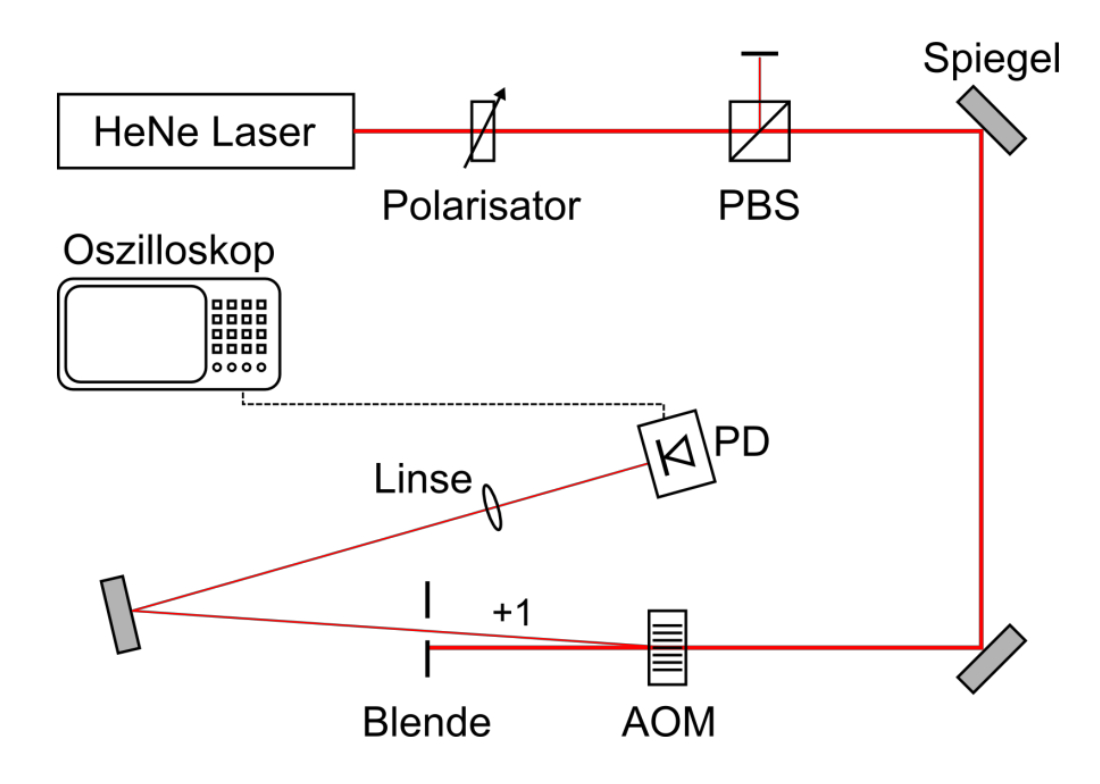
\includegraphics[width=0.7\textwidth]{img/inbetriebnahme.jpg}
  \caption[Cap for listoffigures]{Aufbau zur Detektierung der ersten Beugungsordnung \cite{Anleitung}}
  \label{fig:Bild0}
\end{figure}

Alle Komponenten werden nacheinander so ausgerichtet, dass der Strahl durchgehend möglichst auf der gleichen Höhe (ca. 10 cm) horizontal über dem Tisch verläuft. Bei Installation einer Komponente wird zunächst der Strahl abgeblockt und sichergestellt, dass keine unkontrollierten Reflexe auftreten. Um den Versuchsaufbau nicht zu groß werden zu lassen, wird der Strahl mehrfach mit Spiegeln umgelenkt. Die Linse ist notwendig, um den leicht divergenten Strahl vollständig auf die Fläche der Photodiode abbilden zu können. Mittels der Blende blockieren wir die nullte Beugungsordnung sowie die höheren Beugungsordnungen, so dass die Messung mit dem Photodetektor nur die erste Ordnung erfasst.

Aufällig ist sofort, dass nicht nur die erste Beugungsordnung auftritt, sondern mindestens noch die zweite Ordnung sichtbar ist. Gemäß den Ausführungen zu den Betriebsregimes eines AOMs handelt es sich also nicht um ein (reines) Bragg-Regime. Trotzdem wird das Braggsche Gesetz zugrunde gelegt, da wir vermuten, dass die Abweichung, wenn vorhanden, hinreichend gering ist. Darauf wird später zurückblickend eingegangen.

\section{Beugungseffizienz in Abhängigkeit der Schallintensität}

Es soll nun die Beugungseffizienz $\epsilon = \frac{I_1}{I_{einfallend}}$, d.h.\ der Quotient aus der Intensität des ersten Beugungsmaximums und der gesamten einfallenden Intensität, in Abhängigkeit der Schallintensität bestimmt werden. Dazu wird der Messaufbau unverändert gestartet, wobei nun über ein eigens geschriebenes Computerprogramm die Frequenzgeneratoren und das Oszilloskop derart angesteuert werden, dass jeweils für eine feste Spannung $U_F$ eine Variation von $U_M$ in 0,1 V-Schritten von 0 V bis 5 V erfolgt und die Werte ausgezeichnet werden. $U_F$ verstellen wir von Hand in 1 V-Schritten von 0 V bis 10 V, so dass wir 10 Messreihen mit Werten für die Intensität der ersten Beugungsordnung erhalten. Zu beachten ist das unterschiedliche Offset der Photodiode, welches ohne Streulicht stets 12 mV beträgt und mit Streulicht 16 mV für die zweite Messreihe und 160 mV für alle anderen Messreihen. Dies kommt durch das bei der zweiten Messreihe geschlossene Rollo im Versuchsraum zustande (bedingt durch die Messung einer anderen Laborgruppe). Zusätzlich ist der Laser thermisch nicht völlig stabil, was sich in einer Schwankung des Messwertes für die nullte Begungsordnung von 7,6 V bis 8,16 V bemerkbar macht. Die Spannungsmesswerte, die die Photodiode liefert, sind dabei proportional zur Intensität des Lichtes.

\begin{figure}[h]
\begin{tikzpicture}
\begin{axis}[
  title={Beugungseffizienz $\varepsilon$ für $U_F=0V$},
  epsilonforuf,
  name=first
]
\addplot[red, only marks, mark=x, mark size=2pt, error bars/.cd, y dir=both, y fixed relative=0.07] table[x index=0,y expr=(\thisrowno{1}-0.160)/7.88] {data/Aufgabe3/0V UF.txt};

\addlegendentry{Beugungseffizienz}
\end{axis}

\begin{axis}[
  title={Beugungseffizienz $\varepsilon$ für $U_F=10V$},
  epsilonforuf,
  name=second,
  at=(first.outer south east),
  anchor=outer south west
]
\addplot[red, only marks, mark=x, mark size=2pt, error bars/.cd, y dir=both, y fixed relative=0.07] table[x index=0,y expr=(\thisrowno{1}-0.16)/7.88] {data/Aufgabe3/10V UF.txt};
\addlegendentry{Beugungseffizienz}
\end{axis}
\end{tikzpicture}
\captionof{figure}{$\varepsilon\left(U_m\right)$ für Amplitudenspannungen von 0V und 10V. An Hand dieser Graphen ist noch keine Zusammenhang zwischen $U_F$ und $\varepsilon$ zu erkennen.}
\end{figure}

\begin{figure}[h]
\begin{tikzpicture}
\begin{axis}[
  title={Beugungseffizienz $\varepsilon$ für verschiedene $U_F$},
  epsilonforuf,
  name=first,
  width=0.9\linewidth
]
\addplot[red, only marks, mark=x, mark size=2pt, error bars/.cd, y dir=both, y fixed relative=0.07] table[x index=0,y expr=(\thisrowno{1}-0.160)/7.88] {data/Aufgabe3/0V UF.txt};
\addlegendentry{$U_F = 0V$}
\addplot[blue, only marks, mark=x, mark size=2pt, error bars/.cd, y dir=both, y fixed relative=0.07] table[x index=0,y expr=(\thisrowno{1}-0.160)/7.88] {data/Aufgabe3/5V UF.txt};
\addlegendentry{$U_F = 5V$}
\addplot[black, only marks, mark=x, mark size=2pt, error bars/.cd, y dir=both, y fixed relative=0.07] table[x index=0,y expr=(\thisrowno{1}-0.160)/7.88] {data/Aufgabe3/10V UF.txt};
\addlegendentry{$U_F = 10V$}
\end{axis}

\end{tikzpicture}
\captionof{figure}{$\varepsilon\left(U_m\right)$ für $U_F$ von 0V, 5V und 10V. Hier ist gut zu sehen, dass alle auftreten Intensitätsänderungen innerhalb der Fehlerbalken liegen.}
\end{figure}

\begin{figure}[h]
\begin{tikzpicture}
\begin{axis}[
  title={Maximale Beugungseffizienz $\varepsilon$ in Abh.\ der Amplitudenspannung},
  epsilonforuf,
  name=first,
  width=0.9\linewidth,
  xlabel=$U_F$  in  $V$,
  ylabel=$\varepsilon_{max}$,
  xmax=10,
  ymin=0.6,
  ymax=0.87,
  legend pos=south west
]
\addplot[red, only marks, mark=x, mark size=2pt, error bars/.cd, y dir=both, y fixed relative=0.07] table[x index=0,y expr=(\thisrowno{1}-0.160)/7.88] {data/Aufgabe3/maxima.txt};
\addlegendentry{$\varepsilon_{max}$}
\end{axis}

\end{tikzpicture}
\captionof{figure}{Maximale Beugungseffizienz $\varepsilon_{max}(U_F)$. Die Fehlerbalken aller gemessenen Werte überlappen einander, es ist keine Korrelation zwischen $U_F$ und Beugungseffizienz zu erkennen.}
\end{figure}
\FloatBarrier

Anhand der aufgenommenen Daten ist keine Korrelation zwischen angelegter Amplitudenspanung und auftretender Beugungseffizienz für das erste Maximum zu erkennen. Die auftretende periodische Schwankung in der gemessenen Effizienz ist durch die thermische Instabilität und die damit einhergehende Intensitätsschwankung des verwendeten Lasers zu erklären. Der Intensitätsverlauf des LAsers ist dabei ansatzweise periodisch. Es ist anzumerken, dass sowohl vor als auch nach der Messung mit $U_F = 4V$ eine kurze Pause in der Messreihe eingelegt wurde, was den etwas größeren Sprung in der gemessenen Intensität im Vergleich zu den umliegenden Messungen erklärt.

\section{Beugungseffizienz in Abhängigkeit des Winkels}

Die Messung ist prinzipiell die gleiche wie zuvor, allerdings ist die zu variierende Größe nun der Winkel zwischen Schall- und Lichtwellen und die Spannungen $U_M$, $U_F$ sind konstant. Wir bestimmen zunächst über den Rückreflex des AOMs den Winkel zwischen einfallendem und reflektiertem Strahl, indem ein Schirm mit aufgeklebtem Millimeterpapier direkt neben den einfallenden Strahl zwischen dem letzten Spiegel und AOM aufgestellt wird (für eine gute Genauigkeit möglichst weit vom AOM entfernt). Gemäß folgender Skizze lässt sich der Winkel $\omega$ dann leicht zu $\omega = arc tan (\frac{x}{d})$berechnen: 

\begin{figure}[H] 
  \centering
     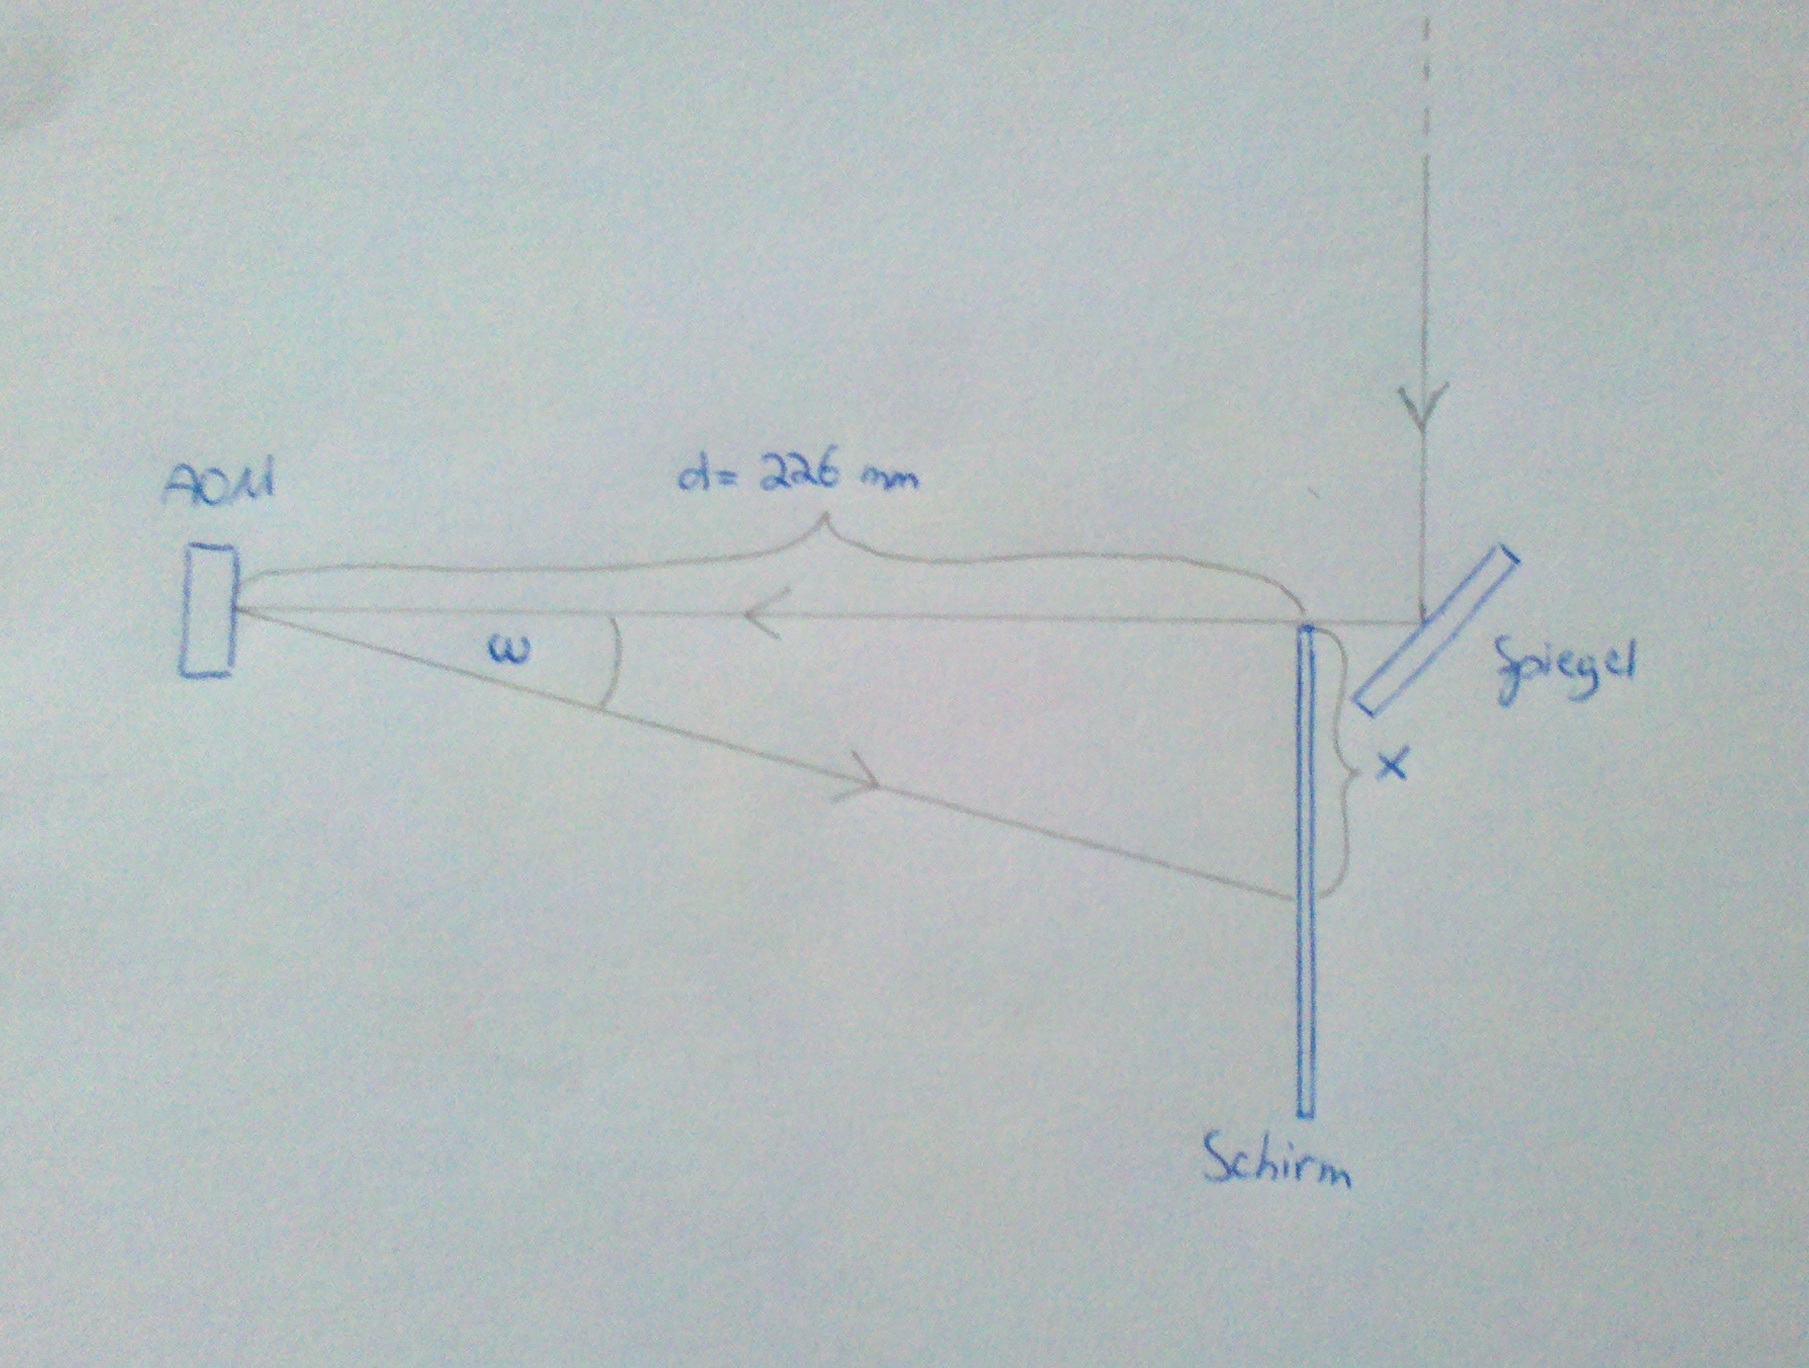
\includegraphics[width=0.7\textwidth]{img/omega-bestimmung.jpg}
  \caption[Cap for listoffigures]{Aufbau zur Winkelbestimmung}
  \label{fig:Bild1}
\end{figure}

Aus der Bragg-Bedingung lässt sich erkennen, dass der Winkel $\theta$ zwischen Schall- und Lichtwellen genau $\frac{\omega}{2}$ ist. D.h.\ $\theta = \frac{arc tan (\frac{x}{d})}{2}$. Die eigentliche Messung erfolgt jeweils nach der Bestimmung von x, wobei dies durch die Größe des Laserstrahls auf dem Schirm erschwert worden ist. Wir setzen daher einen Fehler von $\Delta~x = 0,25~mm$ an.\ d ist konstant mit $d = 226~mm \pm 2~mm$, $U_M = 5~V$ und $U_F = 10~V$. Das Offset beträgt für alle Messungen 16 bzw.\ 12 mV (siehe vorheriger Abschnitt). Um eine bessere Genauigkeit zu erreichen, sind zwei komplette Messreihen von x=0 mm bis x=6,5 mm in Schritten von 0,5 mm aufgenommen worden. Dies entspricht der Detektierung von 2 Maxima.


\begin{figure}[h]
\begin{tikzpicture}
\begin{axis}[
  title={$\varepsilon(\theta)$, gemessen von Esra Bauer},
  epsilonfortheta,
  name=first
]
\addplot[
  red, only marks, mark=x, mark size=2pt, 
  error bars/.cd,
  y dir=both, y fixed relative=0.045,
  x dir=both, x fixed=0.0315
]
table[
  x expr=atan(\thisrow{Abstand}/226)/2,
  y expr=\thisrow{Esra}/6.88
] {data/Aufgabe4/Manuelle Messung.txt};
\addlegendentry{Beugungseffizienz}
\end{axis}

\begin{axis}[
  title={$\varepsilon(\theta)$, gemessen von Sören Link},
  epsilonfortheta,
  name=second,
  at=(first.outer south east),
  anchor=outer south west
]
\addplot[
  red, only marks, mark=x, mark size=2pt,
  error bars/.cd,
  y dir=both, y fixed relative=0.045,
  x dir=both, x fixed=0.0315
]
table[
  x expr=atan((\thisrow{Abstand} + 0.5)/226)/2,
  y expr=\thisrow{Soeren}/6.88
] {data/Aufgabe4/Manuelle Messung.txt};
\addlegendentry{Beugungseffizienz}
\end{axis}
\end{tikzpicture}

\captionof{figure}{2 Messreihen für $\varepsilon(\theta)$, durchgeführt von Esra Bauer und Sören Link. Auf Grund eines gewissen Interpretationsspielraumes beim Ablesen der Messwerte, begründet in der räumlichen Ausdehnung des Laserreflexs in Relation zur notwendigen Häufigkeit der Messungen, wird der Fehler für die Position des Reflexes als relativ groß angenommen. Bei der Messung von Sören Link kommt zu den im Anhang zu findenden original-Messdaten noch ein Offset von $0.5mm$ (entspricht etwa $1,3$°) hinzu, welcher in den Graphen allerdings schon berücksichtigt ist.}

\end{figure}
\FloatBarrier

Ahhand der aufgenommenen Daten ist trotz der Verschiebung, die auf Grund systematischer Fehler zwischen den beiden durchgeführten Messreihen zustande kommt, ein qualitativ eindeutiger Verlauf zu erkennen. So ist die Beugungseffizienz bei 0° zunächst sehr gering, erreicht bei einem Einfallswinkel $\theta$ von etwa 0.25°-0.3° ein Maximum und fällt anschließend wieder ab. Ein zweites Maximum ist bei einem Einfallswinkel um 0.7° zu finden.

Mit Hilfe der Bragg-Bedingung $sin\left( \theta \right) = \frac{\lambda}{2\lambda_s} = \frac{\lambda \cdot \nu_s}{2 v_s}$ lässt sich nun aus den gemessenen Peaks die Schallgeschwindigkeit im AOM ausrechnen.

Für den Winkel $\theta$ benutzen wir hier die Position des ersten Peaks, $\theta = (0,325 \pm 0,0315)$°. Die verwendete Schallfrequenz haben wir auf $\nu_s\left( U_F= 10V \right) = \left( 94,35 \pm 1,8 \right)MHz$ bestimmt. Dies gibt uns eine Schallgeschwindigkeit von $v_s = 4042m/s \pm 519/s$. Der Literaturwert für die Schallgeschwindigkeit im Kristall beträgt $4200m/s$, was von unserer Messung bestätigt werden konnte.

Durch einen Betrieb des AOMs bei einer Frequenzmodulationspannung $U_F$ von $0V$ statt $10V$ wäre durch die geringere Schallfequenz wohl ein genaueres ablesen der Werte möglich gewesen.

\section{Pulserzeugung}

Wir nutzen nun die Möglichkeit, mit dem AOM Laserpulse zu erzeugen. Dazu wird mit den Funktionsgeneratoren eine Pulsspannung in den Modulationseingang eingespeist. Zunächst bleibt der Aufbau so wie in Abbildung 3.1. gezeigt und es werden drei Pulse erzeugt, die sich jeweils in Pulslänge und Repetitionsrate unterscheiden. Diese werden über den Photodetektor aufgezeichnet und auf dem Oszilloskop sichtbar gemacht, wodurch wir die tatsächliche Repetitionsrate, die Pulslänge sowie die Anstiegszeit ablesen können. Die Ergebnisse werden zur Auswertung an den PC übertragen.

\begin{figure}[H]
  \centering
  \begin{subfigure}[h]{0.3\textwidth}
    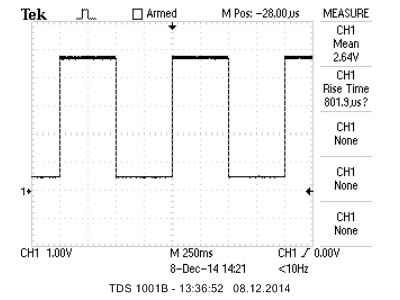
\includegraphics[width=\textwidth]{data/Aufgabe5/1Hz-500ms.png}
    \caption[Cap for listoffigures]{$\tau_P = 500ms$, $f_{rep} = 1Hz$}
    \label{fig:1Hz500ms}
  \end{subfigure}%
  \begin{subfigure}[h]{0.3\textwidth}
    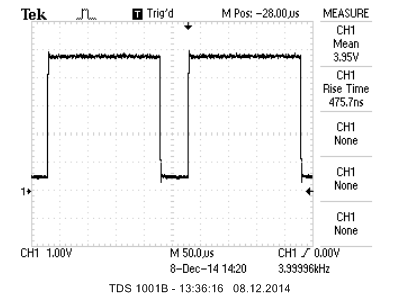
\includegraphics[width=\textwidth]{data/Aufgabe5/4kHz-200us.png}
    \caption[Cap for listoffigures]{$\tau_P = 200\mu s$, $f_{rep} = 4kHz$}
    \label{fig:4kHz200ys}
  \end{subfigure}
  \begin{subfigure}[h]{0.3\textwidth}
    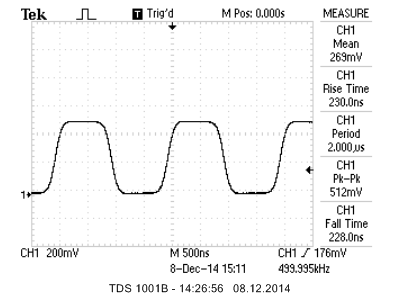
\includegraphics[width=\textwidth]{data/Aufgabe5/500kHz-1us.png}
    \caption[Cap for listoffigures]{$\tau_P = 1\mu s$, $f_{rep} = 500kHz$}
    \label{fig:500kHz1ys}
  \end{subfigure}
  \caption{Oszillioskop-Bilder für unterschiedliche Pulsdauer $\tau_P$ und Frequenzen $f_{rep}$ Am letzten Bild ist bereits deutlich zu erkennen, dass der AOM eine nicht verschwindene Anstiegszeit besitzt.}\label{fig:nolenspulses}
\end{figure}

Es zeigt sich, dass exakte Rechteckpulse nur bis zu einer gewissen Pulsdauer erzeugt werden können; wird diese zu gering, so verformt sich das Rechtecksignal in Richtung einer Sinuskurve. Die Anstiegszeit (in der Grafik als rise time bezeichnet) kann also nicht beliebig klein werden und ist dafür verantwortlich, dass bei einer sehr hohen Frequenz (im Bild bei 500 kHz) der Anstieg deutlich verzögert erfolgt.

Als nächstes werden Pulslänge und Anstiegszeit konstant gewählt: $\tau_P = 1~\mu s$, $t_{rise} = 20~ns$. Der Aufbau wird verändert, so dass er folgender Skizze entspricht:

\begin{figure}[H] 
  \centering
     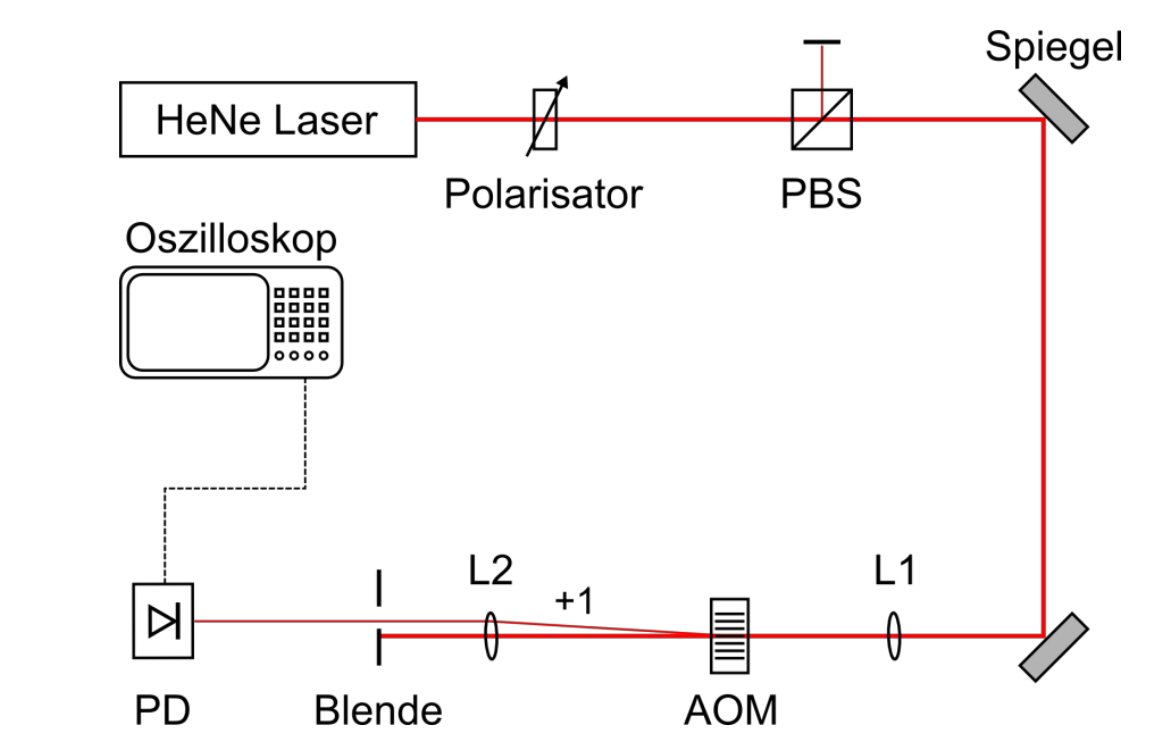
\includegraphics[width=0.7\textwidth]{img/pulserzeugung.jpg}
  \caption[Cap for listoffigures]{Aufbau zur Pulserzeugung mit verschiedenen Linsen L1 und L2 \cite{Anleitung}}
  \label{fig:Bild2}
\end{figure}
\FloatBarrier

Die Messung wird via Oszilloskop für Kombinationen von Linsen L1 und L2 verschiedener Brennweiten ausgewertet und wie vorher aufgezeichnet.

Die Anstiegszeit des gemessenen Laserpulses kommt durch die räumliche Ausdehnung des Lasers im AOM zustande, da das Schallwellengitter sich im Kristall mit Schallgeschwindigkeit bewegt und somit eine gewisse Zeit benötigt, bis es den Laserstrahl komplett erfasst hat. Es ist also ein linearer Zusammenhang zwischen Strahldurchmesser im AOM und Anstiegszeit des gemessenen Laserpulses zu erwarten.

Anfänglich wurde ein Fehler bei der Justierung der Linsen gemacht, insbesondere wurde die im Strahlengang weiter hinten befindliche Linse zu weit vom AOM entfernt angebracht. Aus diesem Grund liegen uns nur 2 verwertbare Messungen vor:

\begin{table}[H]
  \begin{center}
    \begin{tabular}{|p{5cm}|p{4cm}|p{4.5cm}|}
      \hline
          Anstiegszeit in $ns$ & Brennweite L1 in mm & Brennweite L2 in mm \\ \hline
          32.80                & 50                  & 150                 \\ \hline
          42.20                & 200                 & 150                 \\ \hline
    \end{tabular}
  \end{center}
  \caption{Anstiegszeiten des Laserpulses für verschiedene Linsenkombinationen. }
\end{table}
\FloatBarrier

Zwar ist eine Verringerung der Anstiegszeit für eine geringere Brennweite in L1 aus den Daten zu sehen, allerdings macht die Tatsache, dass uns nur 2 Messwerte vorliegen, eine genaue Auswertung unmöglich. Wir sind lediglich in der Lage, einen qualitativen Zusammenhang zwischen einer Verringerung der Brennweite in L1 und dem Strahldurchmesser und somit der Anstiegszeit des Laserpulses zu zeigen.

\section{AOM als Frequenzschieber}

Der AOM soll nun in der Doppelpasskonfiguration in Betrieb genommen werden, um ein Spektrum des Lichtes zu erhalten, welches ihn zweimal passiert hat. Folglich wird der Spektralanalysator an den Photodetektor angeschlossen und die Messapparatur wie folgt aufgebaut: 

\begin{figure}[H] 
  \centering
     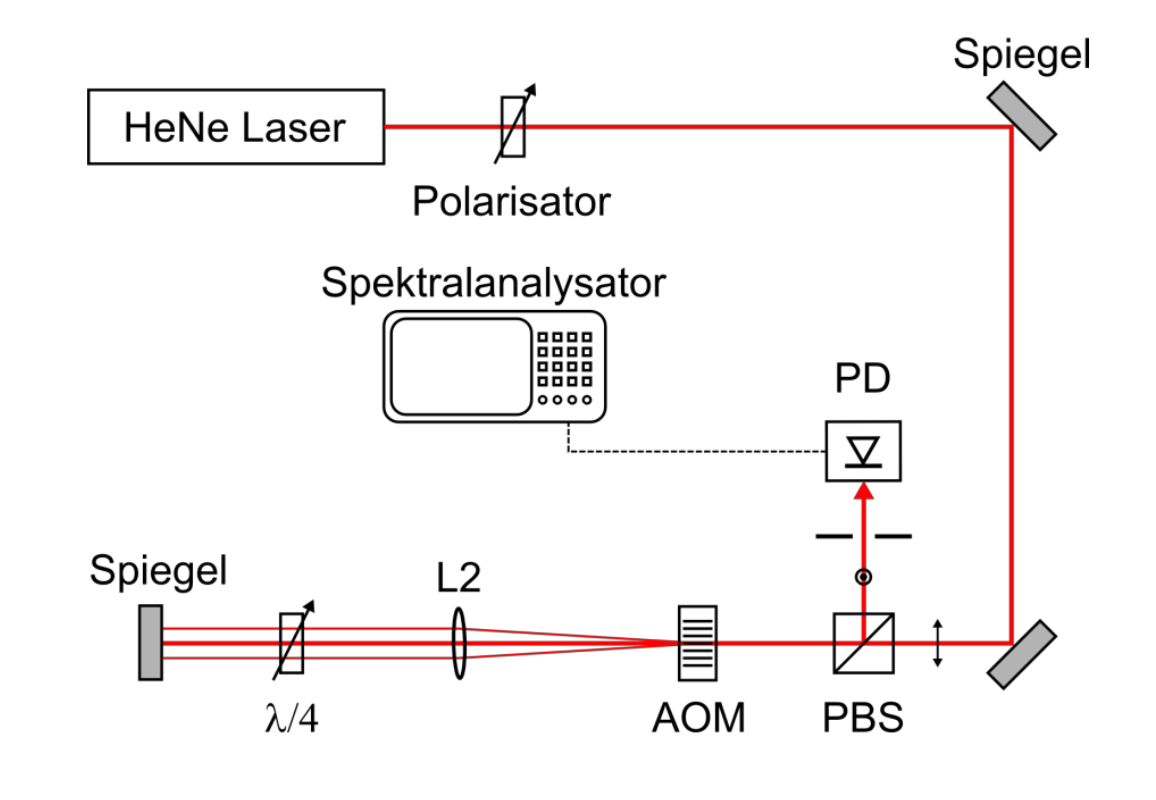
\includegraphics[width=0.7\textwidth]{img/doppelpass.jpg}
  \caption[Cap for listoffigures]{Doppelpasskonfiguration \cite{Anleitung}}
  \label{fig:Bild3}
\end{figure}

Nun wird die Messung mit $U_M = 5~V$ und variabler $U_F$ gestartet. Wir stellen fest, dass die Auflösung der Photodiode nicht ausreicht um die charakteristischen Peaks zu detektieren. Um dennoch die Auswertung dieses Versuches abschließen zu können, wurden uns für diesen Abschnitt Messdaten der Praktikumsgruppe vom 01.12.2014 zur Verfügung gestellt.

\begin{figure}[H]
  \centering
     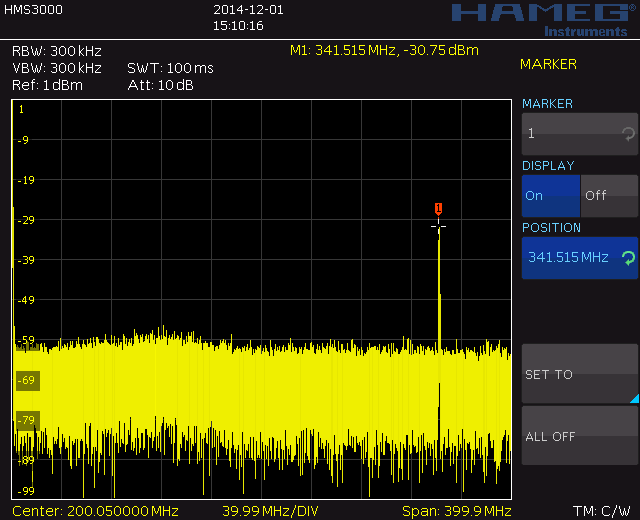
\includegraphics[width=0.7\textwidth]{data/Aufgabe6/aom_aus.png}
  \caption[Cap for listoffigures]{Doppelpassmessung bei ausgeschaltetem AOM. Obwohl keine Frequenzverschiebung durch den AOM auftritt, ist ein Peak bei 341.5 MHz zu sehen.\cite{AndereGruppe}}
  \label{fig:Bild4}
\end{figure}

Offensichtlich treten auch ohne Einwirkung des AOMs Schwebungen zwischen verschiedenen Laserfrequenzen auf. Erklärt werden kann dies durch Schwebung der Grundmode mit höheren im Laser entstehenden longitudinalen Moden. Der Frequenzunterschied zweier benachbarter Lasermoden ist durch $\Delta \nu = \frac{c}{2L}$ gegeben. Einsetzen der Frequenzdifferenz von $341,515 MHz$ ergibt eine theoretische Resonatorlänge von etwa $41,5 cm$. Leider sind uns keine genauen Angaben zur tatsächlichen Resonatorlänge bekannt, allerdings passt der errechnete Wert in etwa zur Größe des verwendeten Lasers.

Bei Inbetriebnahme des AOMs kommen wie erwartet weitere Peaks hinzu.

\begin{figure}[H]
  \centering
  \begin{subfigure}[H]{0.45\textwidth}
    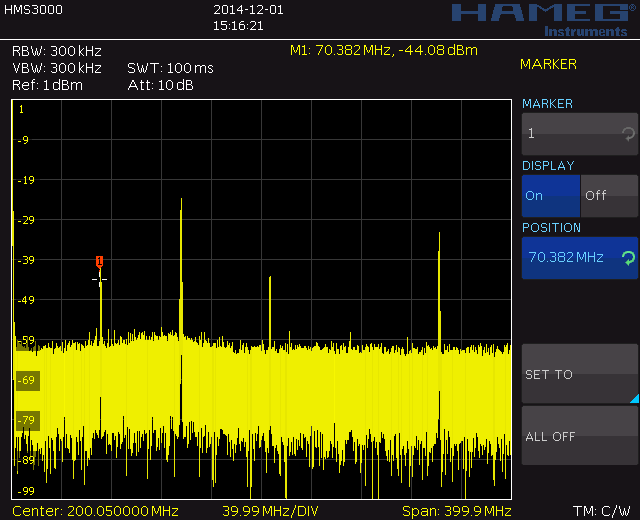
\includegraphics[width=\textwidth]{data/Aufgabe6/frequ_Uf_1.png}
    \caption[Cap for listoffigures]{$U_F = 1V$}
    \label{fig:UF1}
  \end{subfigure}
  \begin{subfigure}[H]{0.45\textwidth}
    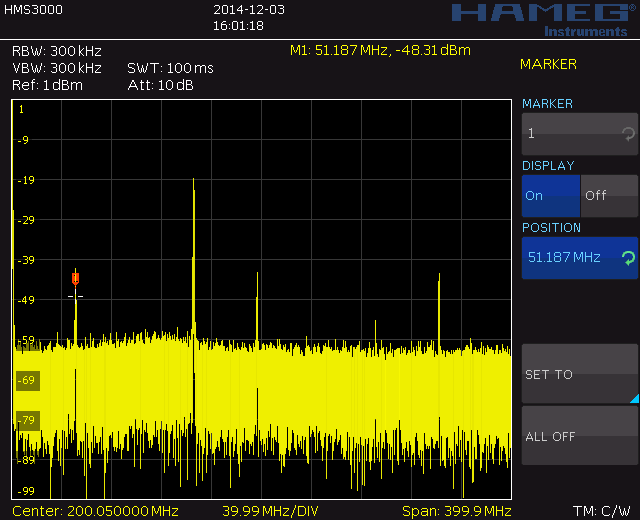
\includegraphics[width=\textwidth]{data/Aufgabe6/Aufgabe6_Uf3V_AOMein.png}
    \caption[Cap for listoffigures]{$U_F = 3V$}
    \label{fig:UF3}
  \end{subfigure}~%
  \caption{Aufgenommene Peaks bei Betrieb des AOMs in Doppelpasskonfugration\cite{AndereGruppe}.}\label{fig:doublepasspeaks}
\end{figure}

Neben dem erwarteten Peak durch die Schwebung der ursprünglichen und der durch den AOM modifizierten Laserfrequenz treten hier noch 2 weitere, schwächere Peaks auf. Es stellt sich heraus, dass der 2. Peak von rechts genau der Frequenzdifferenz zwischen der durch den AOM hervorgerufenen Schwebung und der Lasermoden-Schwebung entspricht, und kann so als Schwebung dieser beiden Frequenzen aufgefasst werden. Der erste Peak von links (abgesehen von dem am Rand zu sehenden Nullpeak) entspricht wiederum genau der Frequenzdifferenz des eben genannten Peaks und des AOM-Peaks.

\begin{table}[H]
  \begin{center}
    \begin{tabular}{|p{3cm}|p{6cm}|}
      \hline
          $U_F$ in V & Position der gemessenen AOM-Peaks \\ \hline
          $1V$       & $136,7 MHz$                       \\ \hline
          $3V$       & $147,1 MHz$                       \\ \hline
    \end{tabular}
  \end{center}
  \caption{Frequenzverschiebung im AOM in Abhängigkeit von der angelegten Frequenzmodulationsspannung \cite{AndereGruppe}. Da wir den Fehler durch die Durchführung nicht beurteilen können, schätzen wir ihn an Hand der Pixelgröße auf $\Delta \nu = 1 MHz$ ab.}
\end{table}

Da der Laser in der Doppelpasskonfiguration den AOM zwei mal durchquert, muss die gemessene Frequenz noch halbiert werden. Anhand dieser Daten kann dann eine Eichung der Frequenzmodulationsspannung $U_F$ durchgeführt werden. 

Da für einen Fit zu wenige Daten vorhanden sind, nehmen wir den Zusammenhang zwischen $\Delta \nu$ und $U_F$ als linear an und erhalten $\nu\left( U_F \right) = 65,75 MHz + \left( 2,6 \pm 0,18 \right)\frac{MHz}{V} \cdot V_F$.


\section{AOM als Deflektor}

Für diese letzte Messung werden beide AOM benötigt, der Strahl wird also horizontal und vertikal abgelenkt. Beide werden so nah wie möglich beieinander aufgestellt, um sie möglichst genau in den Brennpunkt der Linse L2 zu stellen, entsprechend folgender Skizze:

\begin{figure}[H] 
  \centering
     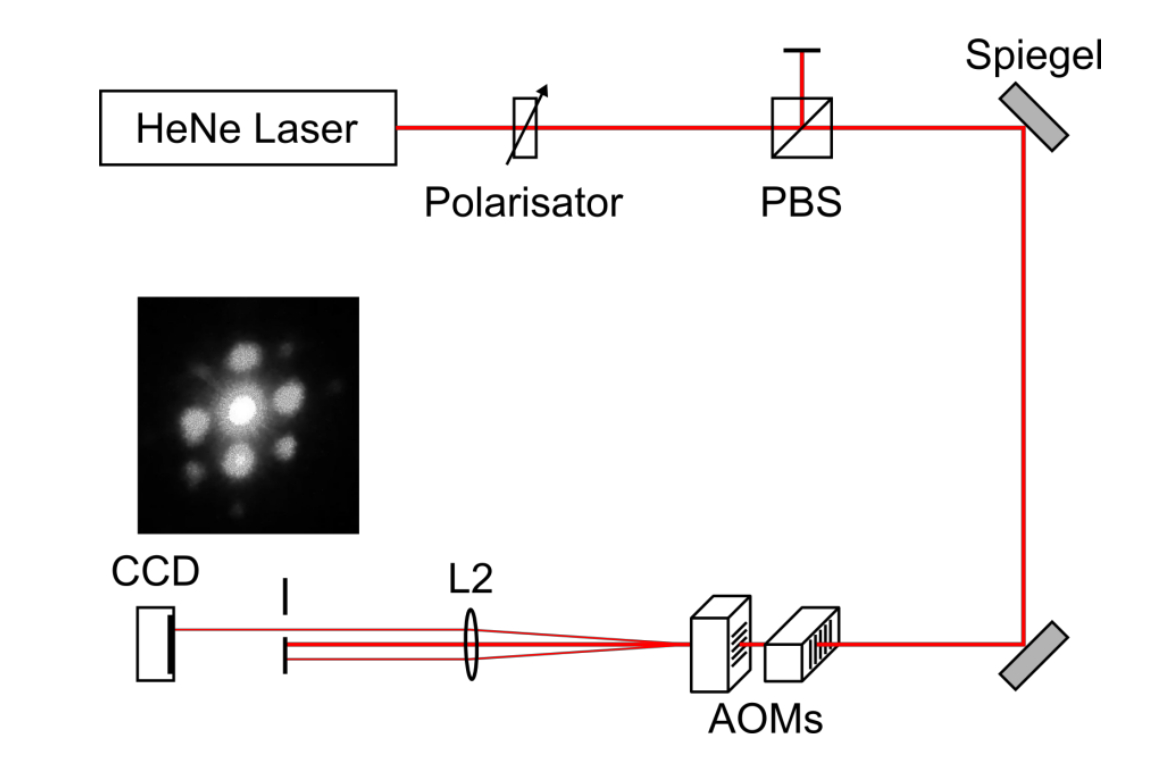
\includegraphics[width=0.7\textwidth]{img/deflektion.jpg}
  \caption[Cap for listoffigures]{Aufbau zur Beobachtung von Lissajous-Figuren \cite{Anleitung}}
\end{figure}

Die Spannung $U_M$ wird für beide AOM konstant auf 5 V eingestellt (sie werden an ein Schaltnetzteil angeschlossen) und $U_F$ wird mit Hilfe der Funktionsgeneratoren derart variiert, dass die Frequenzen mehr oder weniger gering voneinander abweichen. Es wird dabei eine Sinusspannung verwendet, die jedoch stets einen positiven Wert besitzt bzw.\ zwischen 0 V und 10 V liegt. Als Linse L2 setzen wir diejenige mit der größten Brennweite, d.h.\ $f = 200~mm$ ein, da laut Gauß'scher Strahlenoptik durch Linsen mit hohen Brennweiten gebündelte Strahlen eine über einen größeren Abstand annähernd stabile Strahltaille aufweisen. Mittels der CCD Kamera können die entstehenden Lissajous-Figuren sichtbar gemacht und Momentaufnahmen gespeichert werden. Somit wird auch die geringe Ungenauigkeit der Funktionsgeneratoren sofort sichtbar, indem man ein rationales Verhältnis der beiden Frequenzen einstellt und trotzdem eine langsame Rotation der entstehenden Lissajous-Figur beobachtet.


\begin{figure}[H]
  \centering
  \begin{subfigure}[h]{0.32\textwidth}
    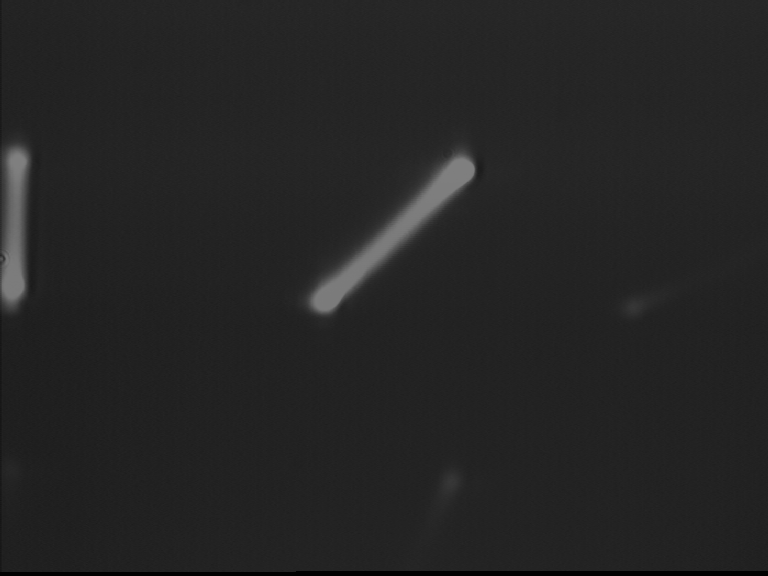
\includegraphics[width=\textwidth]{data/Aufgabe7/1-1-0.png}
    \caption[Cap for listoffigures]{Aufnahme 1}
  \end{subfigure}~%
  \begin{subfigure}[h]{0.32\textwidth}
    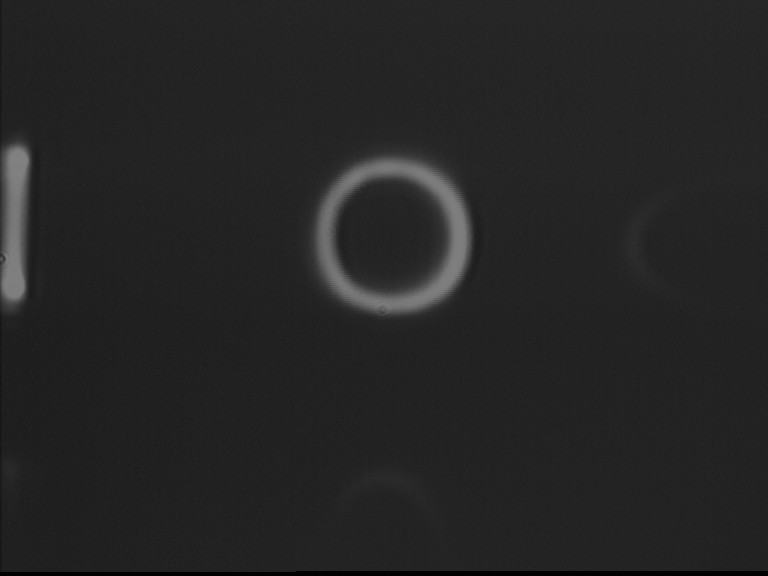
\includegraphics[width=\textwidth]{data/Aufgabe7/1-1-90.png}
    \caption[Cap for listoffigures]{Aufnahme 2}
  \end{subfigure}~%
  \begin{subfigure}[h]{0.32\textwidth}
    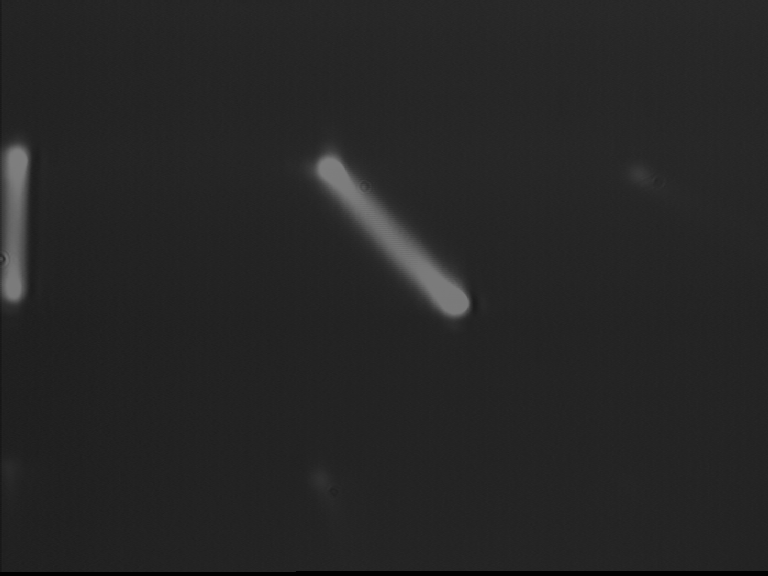
\includegraphics[width=\textwidth]{data/Aufgabe7/1-1-180.png}
    \caption[Cap for listoffigures]{Aufnahme 3}
  \end{subfigure}%
  \caption{Lissajous-Figuren für ein Frequenzverältniss von 1:1}
\end{figure}

\begin{figure}[H]
  \centering
  \begin{subfigure}[h]{0.32\textwidth}
    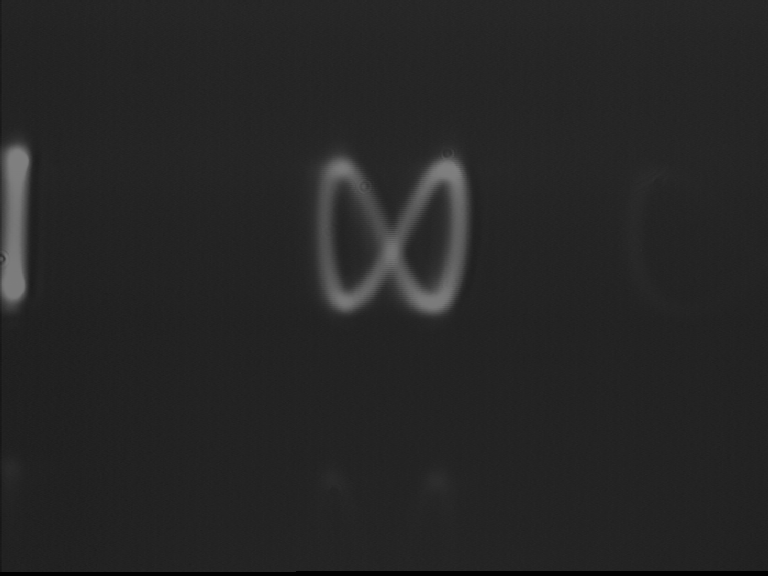
\includegraphics[width=\textwidth]{data/Aufgabe7/2-1-(x-y)halbe.png}
    \caption[Cap for listoffigures]{Aufnahme 1}
  \end{subfigure}~%
  \begin{subfigure}[h]{0.32\textwidth}
    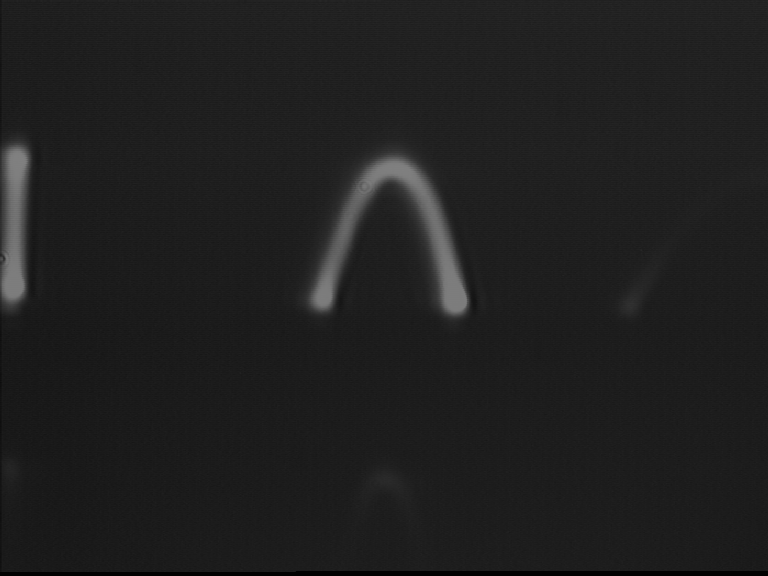
\includegraphics[width=\textwidth]{data/Aufgabe7/2-1-x.png}
    \caption[Cap for listoffigures]{Aufnahme 2}
  \end{subfigure}~%
  \begin{subfigure}[h]{0.32\textwidth}
    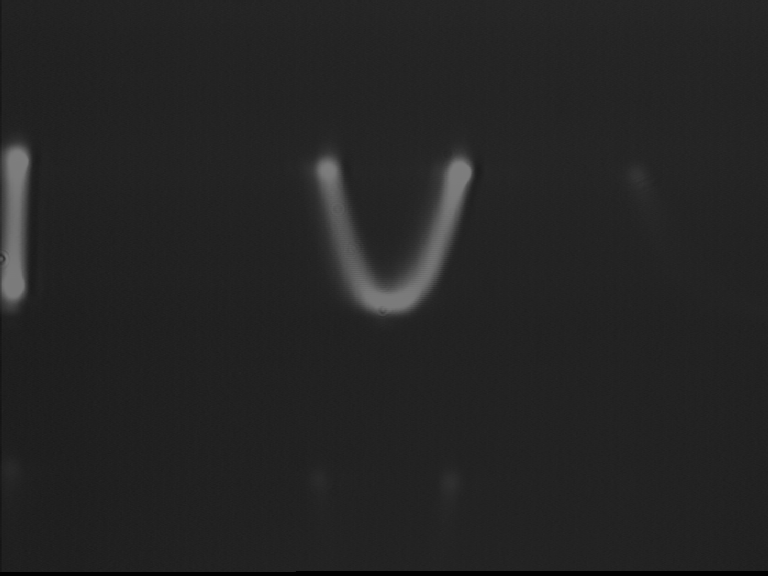
\includegraphics[width=\textwidth]{data/Aufgabe7/2-1-y.png}
    \caption[Cap for listoffigures]{Aufnahme 3}
  \end{subfigure}%
  \caption{Lissajous-Figuren für ein Frequenzverältniss von 2:1}
\end{figure}

\begin{figure}[H]
  \centering
  \begin{subfigure}[h]{0.32\textwidth}
    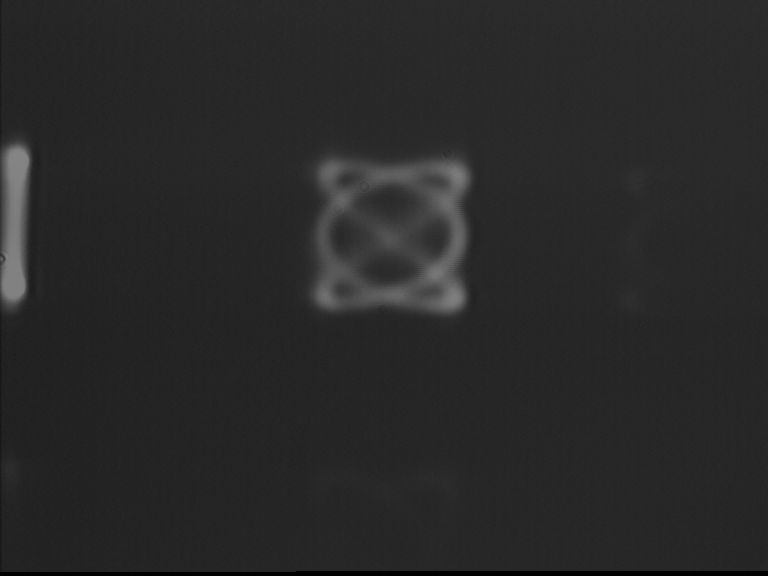
\includegraphics[width=\textwidth]{data/Aufgabe7/2-3-(x-y)halbe.png}
    \caption[Cap for listoffigures]{Aufnahme 1}
  \end{subfigure}~%
  \begin{subfigure}[h]{0.32\textwidth}
    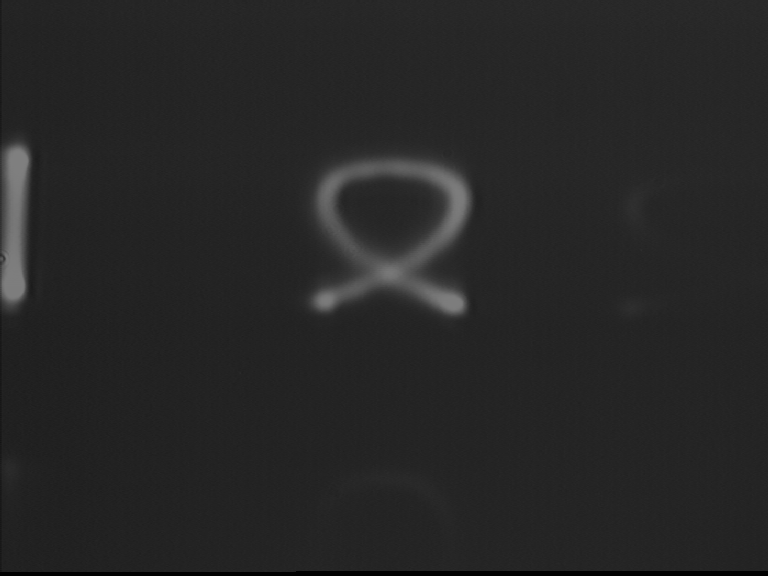
\includegraphics[width=\textwidth]{data/Aufgabe7/2-3-x.png}
    \caption[Cap for listoffigures]{Aufnahme 2}
  \end{subfigure}~%
  \begin{subfigure}[h]{0.32\textwidth}
    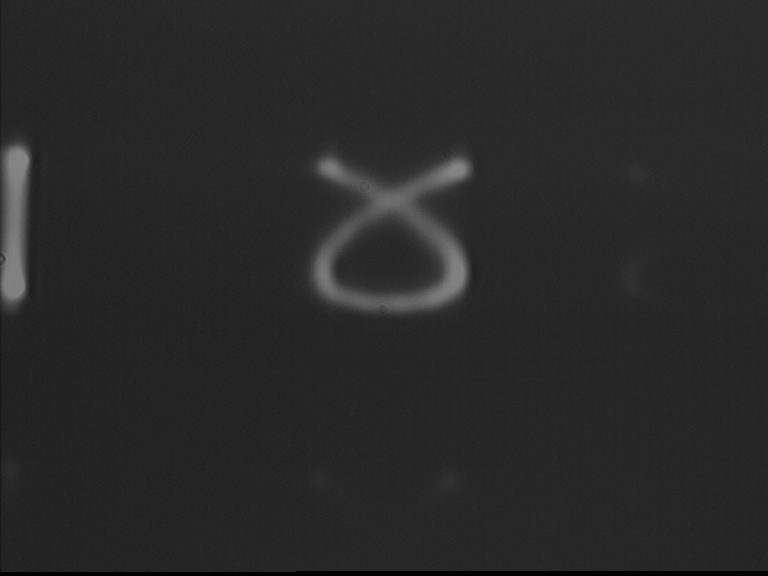
\includegraphics[width=\textwidth]{data/Aufgabe7/2-3-y.png}
    \caption[Cap for listoffigures]{Aufnahme 3}
  \end{subfigure}%
  \caption{Lissajous-Figuren für ein Frequenzverältniss von 2:3}
\end{figure}

\begin{figure}[H]
  \centering
  \begin{subfigure}[h]{0.32\textwidth}
    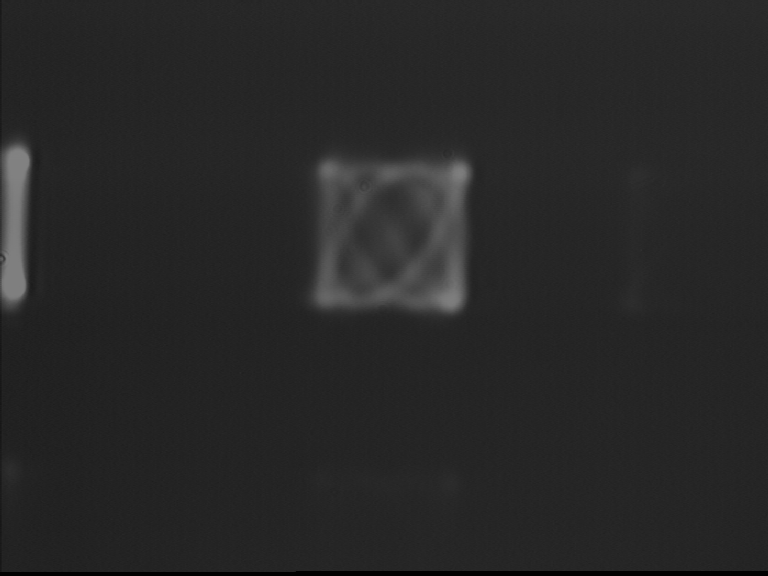
\includegraphics[width=\textwidth]{data/Aufgabe7/4-3-(x-y)halbe.png}
    \caption[Cap for listoffigures]{Aufnahme 1}
  \end{subfigure}~%
  \begin{subfigure}[h]{0.32\textwidth}
    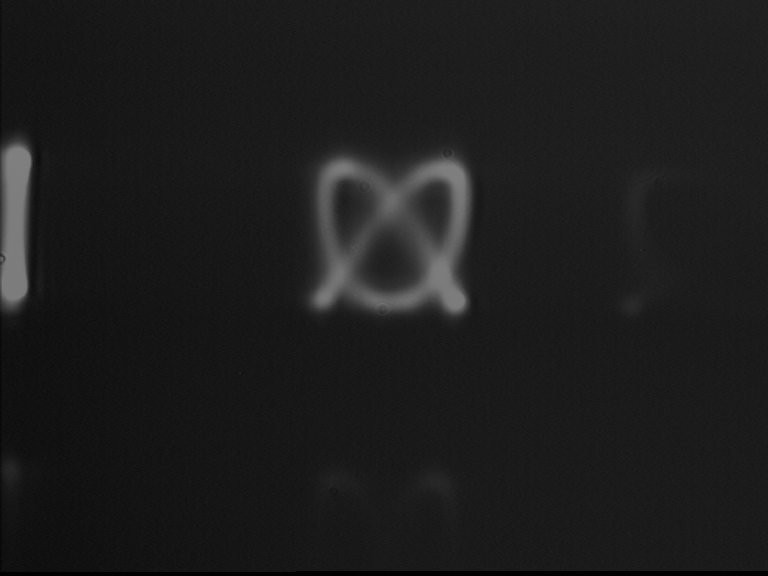
\includegraphics[width=\textwidth]{data/Aufgabe7/4-3-x.png}
    \caption[Cap for listoffigures]{Aufnahme 2}
  \end{subfigure}~%
  \begin{subfigure}[h]{0.32\textwidth}
    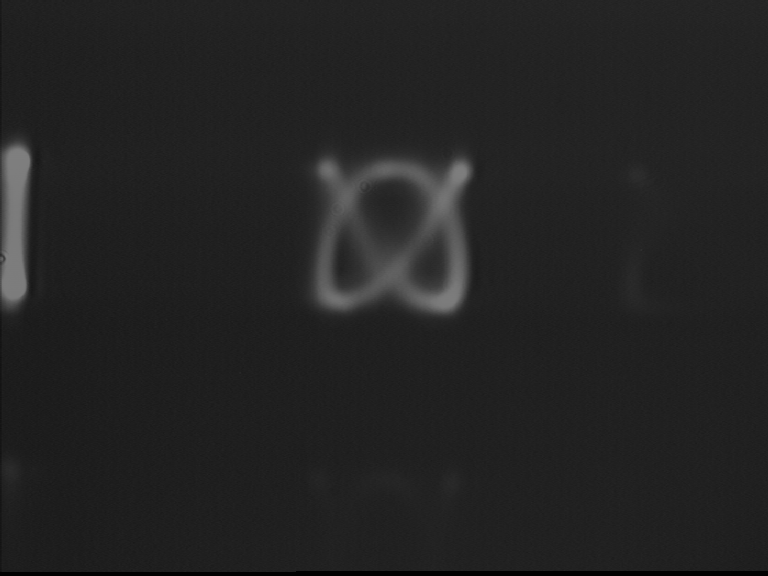
\includegraphics[width=\textwidth]{data/Aufgabe7/4-3-y.png}
    \caption[Cap for listoffigures]{Aufnahme 3}
  \end{subfigure}%
  \caption{Lissajous-Figuren für ein Frequenzverältniss von 4:3}
\end{figure}

Um die unterschiedlichen Phasenverschiebungen zu zeigen, wurden von jeder Einstellung drei Aufnahmen gemacht.


\chapter{Fazit}

In der Tat kann man feststellen, dass die Berechnungen gemäß der Bragg-Bedingung zielführend und von hinreichender Genaugkeit sind, obwohl auch höhere Beugungsordnungen sichtbar gewesen sind. Der exakte Parameter $\rho$ lässt sich leider nicht ohne weiteres berechnen, da schwierig zu bestimmende Größen wie der mittlere Brechnungsindex sowie die Modulation des Brechungsindex enthalten sind. Es ist aber ersichtlich, dass $\rho$ im kritischen Bereich liegen muss, d.h.\ höchstwahrscheinlich zwischen 1 und 10 liegt. Somit lässt sich erklären, dass zwar Beugung nach dem Bragg-Gesetz auftritt, jedoch auch höhere Beugungsordnungen (gemäß des Raman-Nath-Regimes) beobachtet werden können. Dies lässt sich auch mittels des sog. Q-Wertes erklären, der wie folgt definiert ist: 

$$Q = \frac{2 \pi \lambda_L L}{\Lambda^2 n_0}$$,

wobei $\lambda_L$ die Lichtwellenlänge ist, L die Länge des Kristalls im AOM (L kann mit etwa 15 mm abgeschätzt werden), $\Lambda$ die Gitterkonstante (also die Schallwellenlänge im Kristall gemäß $\lambda_S = \frac{v_S}{f_S}$) und $n_0$ der mittlere Brechungsindex, welcher für Tellurdioxid bei 486 nm einen Wert von $n_0 = 2,24$ besitzt \cite{wiki}.

Es ergibt sich für unsere Sitution ein Q-Wert von etwa 11, was der Einschätzung des Parameters $\rho$ entspricht, da ab einem Q-Wert von 10 Bragg-Regime vorliegt und der Q-Wert gerade so darüber liegt, wir können also für die Berechnungen vom Bragg-Regime ausgehen.

%ENDE INHALT
\cleardoublepage{}
% Eintrag fürs Inhaltsverzeichnis
\newpage
\begin{thebibliography}{100}
   \bibitem{GefahrenLaser} \url{http://de.wikipedia.org/w/index.php?title=Laser&oldid=128632514#Gefahren}
   
   \bibitem{Anleitung} Anleitungsblatt zum Versuch
   \bibitem{AndereGruppe} AOM F-Praktikumsgruppe vom 01.12.2014
   \bibitem{wiki} http://de.wikipedia.org/wiki/Tellurdioxid
\end{thebibliography}
\chapter{Messdaten}
\VerbatimInput[label=\fbox{Aufgabe3/0V UF.txt}]{data/Aufgabe3/0V_UF.txt}
\VerbatimInput[label=\fbox{Aufgabe3/1V UF.txt}]{data/Aufgabe3/1V_UF.txt}
\VerbatimInput[label=\fbox{Aufgabe3/2V UF.txt}]{data/Aufgabe3/2V_UF.txt}
\VerbatimInput[label=\fbox{Aufgabe3/3V UF.txt}]{data/Aufgabe3/3V_UF.txt}
\VerbatimInput[label=\fbox{Aufgabe3/4V UF.txt}]{data/Aufgabe3/4V_UF.txt}
\VerbatimInput[label=\fbox{Aufgabe3/5V UF.txt}]{data/Aufgabe3/5V_UF.txt}
\VerbatimInput[label=\fbox{Aufgabe3/6V UF.txt}]{data/Aufgabe3/6V_UF.txt}
\VerbatimInput[label=\fbox{Aufgabe3/7V UF.txt}]{data/Aufgabe3/7V_UF.txt}
\VerbatimInput[label=\fbox{Aufgabe3/8V UF.txt}]{data/Aufgabe3/8V_UF.txt}
\VerbatimInput[label=\fbox{Aufgabe3/9V UF.txt}]{data/Aufgabe3/9V_UF.txt}
\VerbatimInput[label=\fbox{Aufgabe3/10V UF.txt}]{data/Aufgabe3/10V_UF.txt}
\VerbatimInput[label=\fbox{Aufgabe4/Manuelle Messung.txt}]{data/Aufgabe4/Manuelle_Messung.txt}
\cleardoublepage{}
% Eintrag fürs Inhaltsverzeichnis
% Abbildungsverzeichnis einfügen
\end{document}
